% Festlegen des Dokumententyps
\documentclass[a4paper,twoside]{scrartcl}
\addtokomafont{caption}{\footnotesize}

% Papierformat
\usepackage{a4}

% Deutsche Sprache (Silbentrennung, usw.)
\usepackage[ngerman]{babel}
\usepackage[babel,german=quotes]{csquotes}

% Schrifteneinstellungen
\usepackage{lmodern}
\usepackage[T1]{fontenc}
\usepackage{textcomp}

% Kodierung
%\usepackage{ucs}
\usepackage[utf8]{inputenc}

% bessere Matheunterstützung
\usepackage{amsfonts}
\usepackage{amstext}
\usepackage{amsmath}

% Einheiten in Formalen0
\usepackage{siunitx}
\sisetup{%
locale=DE,
scientific-notation = true,
}

% fuer Zitate
\usepackage[natbib=true,style=numeric]{biblatex}
\bibliography{literature}

% Grafiken einbinden
\usepackage{graphicx}

% Grafiken Position erzwingen
\usepackage{here}

% Tabellen
\usepackage{booktabs}

% Verweise in PDF-Dateien
\usepackage
[colorlinks,
pdfstartview = 1,
bookmarksopen = true,
bookmarksnumbered = true,
linkcolor = black,
plainpages = true,
hypertexnames = false,
citecolor = black]{hyperref} 

% PGF einbinden
\usepackage{tikz}
\pgfrealjobname{protocol}
\newcommand{\inputTikZ}[1]{%
    \resizebox{\textwidth}{!}{\input{#1.pgf}}%
  }

\newcommand{\e}{{\rm e}}

\begin{document}

\thispagestyle{empty}
\begin{center}
    {\Huge{\textbf{Physikalisches Praktikum}}}\\[16pt]
\ \\
\ \\
\ \\
\ \\
\ \\
\ \\
\ \\
\ \\
\ \\
\ \\
\ \\
\ \\
\ \\
\ \\
\ \\
\ \\
\ \\
\huge{Kreiselpräzession}
\ \\
\ \\
\large{Versuch 4}
\end{center}

\normalsize
\ \\
\ \\
\ \\
\ \\
\ \\

\begin{center}
\begin{tabular}{lcl}
      Name: & ~ & Timo Janßen \\
                    & ~ & E-Mail: timo.janssen1@stud.uni-goettingen.de \\
	  Mitarbeiter: & ~ & Tom Groß \\
		    & ~ & E-Mail: tom.gross@stud.uni-goettingen.de \\
\ \\		    
      Tutorin: & ~ & Jantje Freudenthal \\
      Gruppe: & ~ & 10 \\
\ \\      
      Durchgeführt am: & ~ & 27.05.2013 \\
      Protokoll abgegeben: & ~ & 10.06.2013 \\
      Protokoll verbessert: & ~ & ........................\\
\ \\
\ \\
      Testiert: .................................    
\end{tabular}\\
\end{center}

\newpage
%Seitennummerierung ausschalten
\thispagestyle{empty}
\tableofcontents
\newpage
%Seitenzähler zurücksetzen
\setcounter{page}{1}
\section{Einleitung}
In diesem Versuch geht es um die Untersuchung der Rotationen eines Kreisels und den sich daraus ergebenden Eigenschaften. Insbesondere die Präzession soll näher betrachtet werden. Kreisel sind alltägliche Gegenstände, ob als Spielzeug oder auch als Messinstrument (zum Beispiel als Gyroskop). Die Bewegungsgleichungen des Kreisels finden insbesondere in der Astronomie Anwendung, wo sie die Bewegungen der Himmelskörper beschreiben.
%\newpage
\section{Theorie}
\subsection{Die gedämpfte erzwungene Schwingung}
In der homogenen Differentialgleichung des gedämpften harmonischen Oszillators gibt es drei wesentliche Größen: Das der
(Winkel-)Beschleunigung entgegenwirkende Trägheitsmoment $\Theta$ (hier das Schwungrad), die zur (Winkel-)Geschwindigkeit proportionale Reibung
$\rho$ und das direkt zur Position (hier der Winkel $\phi$) proportionale Rückstellmoment $D^*$.
Hinzu kommt die Anregung. Diese wird periodisch beschrieben durch $M\cos(\omega t).$ 
Zusammen ergeben diese Faktoren die Bewegungsgleichung des Pohlschen Rades:
\begin{align}
\label{eq:1}
\Theta\ddot{\varphi}+\rho\dot{\varphi}+D^*=M\cos(\omega t)
\end{align}
Um diese Gleichung auf die Normalform einer Bewegungsgleichung für eine gedämpfte Schwingung mit Anregung zu bringen, teilen
wir durch $\Theta$ und erhalten für $\rho/\Theta=:2\beta$, $D^*/\Theta=:\omega_0^2$ und $M/\Theta=:N$
die inhomogene lineare Differentialgleichung 2. Ordnung
\begin{align}
\label{eq:2}
\ddot{\varphi}+2\beta\dot{\varphi}+\omega_0^2\varphi=N\cos(\omega t).
\end{align}


\subsection{Die homogene Differentialgleichung}
\label{h.DGL}
Betrachten wir zunächst die Gleichung des frei schwingenden Rades, also ohne Anregung, so erhalten wir die homogene Differentialgleichung
\begin{align}
\label{eq:3}
\ddot{\varphi}+2\beta\dot{\varphi}+\omega_0^2\varphi=0
\end{align}
welche mit dem Exponentialansatz $\varphi(t)=e^{\lambda t}$ gelöst werden kann. Hier sind die drei Fälle $\beta>\omega_0$, $\beta=\omega_0$ und $\beta<\omega_0$ zu unterscheiden. 
Wir werden uns hier mit dem sogenannten Schwingfall $\beta<\omega_0$ befassen. 
Offensichtlich bekommt hier die Wurzel ein negatives Argument, was zu folgender Lösung für
Gleichung (\ref{eq:3}) führt:
\begin{align}
\label{eq:4}
\varphi(t)=e^{-\beta t}\cdot\left(Ae^{i\sqrt{\omega_0^2-\beta^2}t} + Be^{-i\sqrt{\omega_0^2-\beta^2}t}\right)
\end{align}
Nun ist noch die Anfangsphase $\phi$, sowie die Reellen Zahlen A und B, welche 
in der Ausgangsamplitude $\varphi_0$ zusammengefasst werden zu bestimmen. Setzen wir $A:=\frac{\varphi_0}{2}\cdot e^{i\phi}$ und 
$B:=\frac{\varphi_0}{2}\cdot e^{-i\phi}=\bar{A}$ so erhalten wir \begin{align}
\label{eq:5}
\varphi(t) &= e^{-\beta t}\cdot\left(\frac{\varphi_0}{2}\cdot e^{i\phi}\cdot e^{i\sqrt{\omega_0^2-\beta^2}t} + 
\frac{\varphi_0}{2}\cdot e^{-i\phi}\cdot e^{-i\sqrt{\omega_0^2-\beta^2}t}\right)\nonumber \\
&= e^{-\beta t}\cdot\frac{\varphi_0}{2}\cdot\left(e^{i(\phi+\sqrt{\omega_0^2-\beta^2}t)}+e^{-i(\phi+\sqrt{\omega_0^2-\beta^2}t)}\right).
\end{align}
Mit $\sqrt{\omega_0^2-\beta^2}=:\omega_e$, der Eigenfrequenz des Rades bei der entsprechenden Schwingung, folgt nach der 
\glqq Eulerschen Identität \grqq{} die Schwingungsgleichung für das Pohlsche Rad ohne Antrieb.
\begin{align}
\label{eq:6}
\varphi(t)=\varphi_0\cdot e^{\beta t}\cdot\cos(\omega_e + \phi)
\end{align}

\subsection{Interpretation und logarithmisches Dekrement}
\label{log.Dek}
Der Schwingungsverlauf des Rades ist also cosinus-periodisch und wird um den von der Zeit abhängigen Faktor $e^{-\beta t}$ geschwächt. 
Diese  Dämpfung kann über das logarithmische Dekrement $\Lambda$ beschrieben werden. Dabei gilt:
\begin{align}
\label{eq:7}
\Lambda := \rm {ln}\left[{\frac{\varphi(t)}{\varphi(t+T)}}\right]={\rm {ln}}[e^{\beta T}]=\beta T
\end{align}
Hier beschreibt T die Periodendauer. Das logarithmische Dekrement hängt also lediglich von der Periodendauer, nicht 
von der Zeit ab.

\subsection{Die inhomogene Differentialgleichung}
\label{inh.DGL}
Um die Gleichung der erzwungenen Schwingung zu finden, müssen wir nun die inhomogene Gleichung (\ref{eq:2}) lösen. 
Die Lösung einer inhomogenen Gleichung setzt sich aus der Lösung der zugehörigen homogenen 
Differentialgleichung (\ref{eq:6}) und einer partikulären Lösung zusammen. 
Die partikuläre Lösung erhalten wir durch Einsetzen des Ansatzes $\varphi=\varphi_0\cdot \cos(\omega t-\phi)+c$ in 
(\ref{eq:2}):
\begin{align}
\label{eq:8}
(\omega_0^2-\omega^2)\cdot\varphi_0\cdot\cos(\omega t-\phi)-2\beta\cdot\omega\cdot\sin(\omega t-\phi)+c=N\cos(\omega t). 
\end{align}
Nun müssen $\varphi_0$ und $\phi$ so bestimmt werden, dass die Gleichung für alle Zeiten t erfüllt ist.
Mithilfe der Additionstheoreme gelangt man von dieser Gleichung zu folgenden zwei Bedingungen:
\begin{align}
\label{eq:9}
\varphi_0\cdot\left((\omega_0^2-\omega^2)\cdot\cos(\phi)+2\beta\cdot\omega\cdot\sin(\phi)\right) &= N \\
\label{eq:10}
(\omega_0^2-\omega^2\cdot\sin(\phi) &= 2\beta\cdot\omega\cdot\cos(\phi)
\end{align}
Aus (\ref{eq:10}) folgt direkt die Phasenverschiebung:
\begin{align}
\label{eq:11}
\phi=\arctan\left(\frac{2\beta\omega}{\omega_0^2-\omega^2}\right)
\end{align}
Aus (\ref{eq:9}) lässt sich nach kurzem Umformen und Einsetzen der Phasenverschiebung $\varphi_0$ bestimmen:
\begin{align}
\label{eq:12}
\varphi_0=\frac{N}{(\omega_0^2-\omega^2)^+4\beta^2\cdot\omega^2}
\end{align}
Einsetzen dieses Ergebnisses führt zu folgender partikuläreN Lösung der Schwingungsgleichung (\ref{eq:2}) für die gedämpfte erzwungene Schwingung 
des Pohlschen Rades:
\begin{align}
\label{eq:13}
\varphi(t)=\frac{N}{(\omega_0^2-\omega^2)^+4\beta^2\cdot\omega^2}\cdot\cos\left(\omega t-\arctan\left(\frac{2\beta\omega}{\omega_0^2-\omega^2}\right)\right)
\end{align}
Da die Lösung der homogenen Differentialgleichung für lange Messzeiten gegen Null geht (die Amplitude fällt mit der Exponentialfunktion $e^{-\beta t}$ 
ab), kann für die erzwungene Schwingung bei längeren Schwingzeiten die homogene Gleichung vernachlässigt werden.
Damit beschreibt die partikuläre Lösung der inhomogenen Differentialgleichung die Schwingung für große Zeiten t zunehmend genau. Die Zeit, nach der die homogene Gleichung mit Null angenähert werden kann bezeichnet man als Einschwingvorgang.
\newpage
\subsection{Die Amplitudengleichung}
\label{ampl}
Die Amplitudenstärke
\begin{align}
\label{eq:14}
A(\omega,\beta)=\frac{N}{(\omega_0^2-\omega^2)^2+4\beta^2\cdot\omega^2}
\end{align}
ist gegeben als Vorfaktor der Schwingungsgleichung (\ref{eq:13}) in Abhängigkeit von der Erregerfrequenz $\omega$ und der Dämpfung $\beta$.
Da wir das Resonanzverhalten der Schwingung bei einer bestimmten Dämpfung betrachten wollen, gehen wir jeweils von einem festen $\beta$ aus 
und bestimmen die Amplitude in Abhängigkeit von der Anregung.\\
Dabei ist das Betrachten des Maximums besonders relevant. Dafür berechnen wir die Nullstellen der Ableitung der 
Amplitudengleichung. Die relevante Nullstelle dieser Ableitung ist
\begin{align}
\label{eq:16}
\omega=\sqrt{\omega_0^2-2\beta^2}=:\omega_r.
\end{align}
$\omega_r$ ist die Resonanzfrequenz des Systems. Entspricht die Anregungsfrequenz der Resonanzfrequenz, des angeregten 
Systems, so wird die Schwingsamplitude maximal. In diesem Fall, wird das schwingende System immer weiter angeregt, 
bis es schließlich (abhängig von der Dämpfung) im Extremfall zu einer sogenannten Resonanzkatastrophe
kommt. Als Resonanzkatastrophe wird der Zustand bezeichnet, bei welchem die Amplitude des schwingenden Systems gegen 
unendlich geht. 

\subsection{Phasenverschiebung}
In Kapitel \ref{inh.DGL} wurde die Gleichung (\ref{eq:11}) der Phasenverschiebung
\begin{align}
\phi=\arctan\left(\frac{2\beta\omega}{\omega_0^2-\omega^2}\right) \nonumber
\end{align}
hergeleitet.
Anhand dieser Gleichung ist zu sehen, wie sich unterschiedliche Dämpfungen, beziehungsweise Anregungen auf die 
Phasenverschiebung $\phi$ auswirken.
%\newpage
\section{Durchführung}


%\newpage
\section{Auswertung}
\subsection{Oberflächenspannung}
Für die Berechnung der Oberflächenspannungen wurden zunächst die Durchmesser der Kapillare und die jeweiligen Steighöhen aus den Messungen gemittelt. Es ergeben sich die folgenden Ergebnisse:
\begin{table}[!htbp]
\centering
	\begin{tabular}{l|l}
		\hline
		Kapillare & Durchmesser \\
		\hline \hline
		Grün  & $\SI{1.763(6)e-3}{\m}$  \\
		Blau & $\SI{1.203(6)e-3}{\m}$  \\
		Rot & $\SI{8.27(6)e-3}{\m}$ \\
		\hline
	\end{tabular}
	\caption{Durchmesser der Kapillare}
	\label{tab:1}
\end{table}
\newline
Der Fehler des Durchmessers wurde über
\begin{align*}
\sigma_d = \frac{\sigma_{d_{Messung}}}{\sqrt{n}}
\end{align*}
bestimmt. Dabei ist $n$ die Anzahl der Messungen und es wurde $\sigma_{d_{Messung}} = \SI{1e-5}{\m}$ geschätzt.

Mit der Formel <Link> kann nun die Oberflächenspannung der einzelnen Fluide bestimmt werden. 

\begin{figure}[!htbp]
\begin{center}
	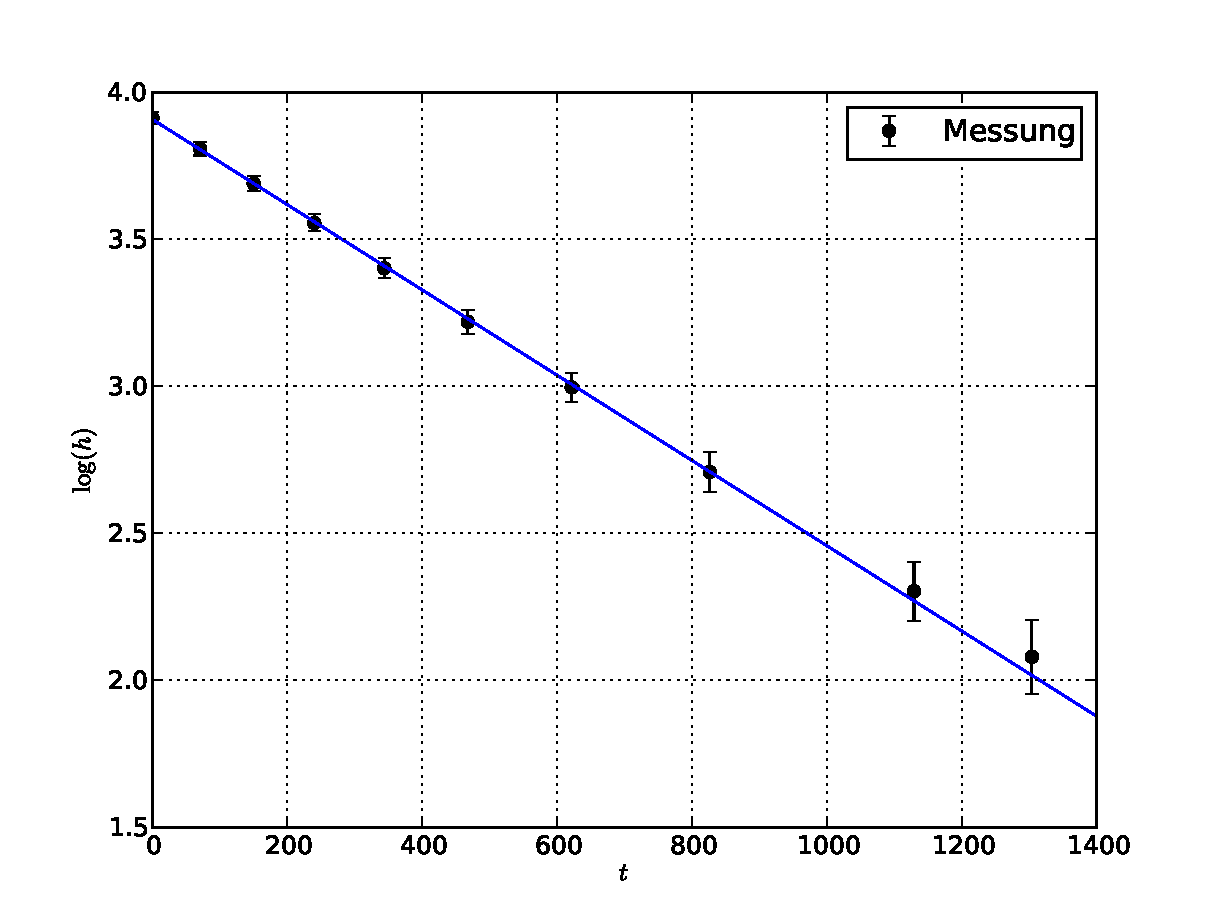
\includegraphics[scale=0.70]{Plot_Aufg2b}
\end{center}
\caption{Auslauf halblogarithmisch aufgetragen}
\end{figure}
%\newpage
\section{Diskussion}
\begin{table}[H]
    \centering
    \footnotesize
    \begin{tabular}{@{}{l}{r}{l}@{$\,=\,$}{l}@{}}
      \toprule
      	Methode & & \multicolumn{2}{l}{Trägheitsmoment} \\
      \midrule
        \multicolumn{2}{l}{Berechnung aus Versuchsparametern} & \multicolumn{2}{c}{} \\
      	 & horizontal & $I_{\text{hor}}$ & $\SI{0,00993}{\kg\m\squared}$ \\
      	 & vertikal & $I_{\text{ver}}$ & $\SI{0.0477\pm0.0005}{\kg\m\squared}$ \\
      \cmidrule{3-4}
      	 & & $\frac{I_{\text{hor}}}{I_{\text{ver}}}$ & $\SI{0,20817610\pm0,00000002}{}$ \\
      \midrule
        \multicolumn{2}{l}{Physikalisches Pendel} & $I_{\text{hor}}$ & $\SI{8,51\pm0,05e-3}{\kg\m\squared}$ \\
      \midrule
        \multicolumn{2}{l}{Präzessionsmessung} & $I_{\text{hor}}$ & $\SI{8,57\pm0,27e-3}{\kg\m\squared}$ \\
      \midrule
        \multicolumn{2}{l}{Nutationsmessung} & $\frac{I_{\text{hor}}}{I_{\text{ver}}}$ & $\SI{0,15\pm0,04}{}$ \\
      \bottomrule
    \end{tabular}%
  \caption{Zusammenfassung der Ergebnisse der Auswertung}
  \label{tab:6}
\end{table}
Der allein mit den Versuchsparametern berechnete Wert für $I_{\text{hor}}$ musste ohne Fehlerintervalle berechnet werden, da zu den Angaben am Versuchsaufbau keine Fehler bekannt sind. Trotzdem sollte dies der theoretisch beste Wert sein, da die Fehler im Vergleich zu den anderen Messmethoden eher klein ausfallen sollten und keine Störeinflüsse die Messung verfälscht haben können.\\
Bei den beiden Werten, die mit dem Pendel und der Präzession gemessen wurden, fällt auf, dass diese zwar gut übereinstimmen, jedoch merklich unter dem erwarteten Wert liegen (vgl. Tab. \ref{tab:6}). Auch die Fehlerintervalle der größten Einzelwerte liegen außerhalb dieses Wertes. Ob hier ein systematischer Fehler vorliegt kann nicht mit Sicherheit gesagt werden, da bei der Berechnung mehrere Vereinfachungen vorgenommen wurden:
\begin{itemize}
	\item \textit{Physikalisches Pendel}: Die verwendete Gleichung gilt nur für kleine Auslenkungswinkel. Zudem wurden 												  die Dämpfung durch Reibung im Lager und die Luftreibung nicht berücksichtigt. 											  Auch wurde das Zusatzgewicht als am Rand des Rades konzentrierte Punktmasse 												  betrachtet, obwohl der Schwerpunkt der Masse tatsächlich weiter außen lag.
	\item \textit{Präzessionsmessung}: Wie beim Pendel wurde keine Reibung berücksichtigt. Der Beitrag des Stabes zum 						  					   Trägheitsmoment wurde vernachlässigt. Außerdem ist die Messung der 														   Präzessionsperiode zwangsläufig ungenau, da die gesamte Messung sehr schnell 											   erfolgen muss, um genügend Messpunkte aufzunehmen, bevor das Zusatzgewicht den 											   Boden berührt.
\end{itemize}
Dies könnte durchaus den nötigen Fehler von etwa 16\% rechtfertigen.\\
Bei der Nutationsmessung liegt der erwartete Wert nur knapp außerhalb des Fehlerintervalls, obwohl das Messverfahren relativ unpräzise wirkt: Die Nutationsperiode muss manuell per Stoppuhr gemessen werden, während die Rotationsfrequenz möglichst groß und der Auslenkungswinkel möglichst klein (um die Kleinwinkelnäherung zu begründen, vgl. Gleichung (\ref{eq:7})) sein sollten. Tatsächlich scheint hier relativ gut gemessen worden zu sein, denn auch die lineare Regression zeigt eine gute Korrelation (vgl. Tab. \ref{tab:4}).\\
Insgesamt sind die Ergebnisse im Rahmen der Messgenauigkeit durchaus zufriedenstellend, wobei die angegebenen Fehler offensichtlich noch nach oben korrigiert werden sollten.
\newpage
\thispagestyle{empty}
% Festlegung Art der Zitierung - Havardmethode: Abkuerzung Autor + Jahr
\printbibliography
\appendix
\section{Messwerte (Original)}
\end{document}